%%%%%%%%%%%%%%%%%%%%%%%%%%%%%%%%%%%%%%%%%
% Stylish Article
% LaTeX Template
% Version 2.1 (1/10/15)
%
% This template has been downloaded from:
% http://www.LaTeXTemplates.com
%
% Original author:
% Mathias Legrand (legrand.mathias@gmail.com) 
% With extensive modifications by:
% Vel (vel@latextemplates.com)
%
% License:
% CC BY-NC-SA 3.0 (http://creativecommons.org/licenses/by-nc-sa/3.0/)
%
%%%%%%%%%%%%%%%%%%%%%%%%%%%%%%%%%%%%%%%%%

%----------------------------------------------------------------------------------------
%	PACKAGES AND OTHER DOCUMENT CONFIGURATIONS
%----------------------------------------------------------------------------------------

\documentclass[fleqn,24pt]{SelfArx} % Document font size and equations flushed left

\usepackage[english]{babel} % Specify a different language here - english by default

\usepackage [autostyle, english = american]{csquotes}
\MakeOuterQuote{"}
%----------------------------------------------------------------------------------------
%	COLUMNS
%----------------------------------------------------------------------------------------

\setlength{\columnsep}{0.55cm} % Distance between the two columns of text
\setlength{\fboxrule}{0.75pt} % Width of the border around the abstract

%----------------------------------------------------------------------------------------
%	COLORS
%----------------------------------------------------------------------------------------

\definecolor{color1}{RGB}{0,0,90} % Color of the article title and sections
\definecolor{color2}{RGB}{0,20,20} % Color of the boxes behind the abstract and headings

%----------------------------------------------------------------------------------------
%	HYPERLINKS
%----------------------------------------------------------------------------------------

\usepackage{hyperref} % Required for hyperlinks
\graphicspath{ {images/} }
\hypersetup{hidelinks,colorlinks,breaklinks=true,urlcolor=color2,citecolor=color1,linkcolor=color1,bookmarksopen=false,pdftitle={Title},pdfauthor={Author}}

%----------------------------------------------------------------------------------------
%	ARTICLE INFORMATION
%----------------------------------------------------------------------------------------

\JournalInfo{29 February 2016} % Journal information
\Archive{} % Additional notes (e.g. copyright, DOI, review/research article)

\PaperTitle{UBC CPSC 416 Distributed Systems: Project Proposal} % Article title

\Authors{Alcuaz, Ito Franchilo Mikael\textsuperscript{1}
| Aziz, Shariq\textsuperscript{2}
| Ko, Mimi\textsuperscript{3}
| Musa, Abrar\textsuperscript{4}
} % Authors
\affiliation{\textsuperscript{1}\textit{y9u8, ialcuaz@alumni.ubc.ca}} % Author affiliation
\affiliation{\textsuperscript{2}\textit{i2u9a, shariqazz15@gmail.com}} % Author affiliation
\affiliation{\textsuperscript{3}\textit{o3d7, mimi@dbzmail.com}} % Author affiliation
\affiliation{\textsuperscript{4}\textit{i1u9a, abrar.musa.89@gmail.com}} % Author affiliation

\Keywords{} % Keywords - if you don't want any simply remove all the text between the curly brackets
\newcommand{\keywordname}{Keywords} % Defines the keywords heading name

%----------------------------------------------------------------------------------------
%	ABSTRACT
%----------------------------------------------------------------------------------------

\Abstract{

Media streaming refers to the constant delivery of time-ordered multimedia content from a server to a client. It is an attractive option as opposed to conventional file transfer methodologies as it provides instant access for the end user and is quite flexible -- a user doesn't have to download the entire file beforehand as was traditionally done in the past, and can interact with the data as it arrives.
Naturally, such a system demands a high bandwidth connection and so works more effectively for users on faster internet networks. This proposal serves as an outline for a possible solution to this key shortcoming by de-centralizing the server-client model through the use of peer-to-peer (P2P) stream networking.
}

%----------------------------------------------------------------------------------------

\begin{document}

\flushbottom % Makes all text pages the same height

\maketitle % Print the title and abstract box

\tableofcontents

\thispagestyle{empty} % Removes page numbering from the first page

%----------------------------------------------------------------------------------------
%	ARTICLE CONTENTS
%----------------------------------------------------------------------------------------

\section{Introduction} % The \section*{} command stops section numbering

A P2P implementation of a media streaming system alleviates some of the bandwidth requirements due to the fact that content is distributed over several streams rather than over one singular server. Usually the content is multicasted from a server to some number of clients which has requested the stream; YouTube makes use of this notion by deploying multiple content delivery networks (CDNs) which distribute the content by demand; the video content is streamed over a single connection, and as such, demands a high bandwidth for maximum playability. The idea behind using P2P streaming is to make the system more scalable -- as the number of clients increase, so do the number of peers which can now make the data available to other clients who also requested the stream (similar to how P2P BitTorrent file sharing works). The server and clients therefore together form a network of media streams.

Chord \cite{2} is a ring-based DHT overlay network which is constructed on top of the usual TCP/IP protocols; this group will examine this implementation primarily and use it as a model for this project using the Go programming language. 

\section{Implementation Strategy}

\subsection{DHT system structure/overlay and file storage}

\begin{figure}
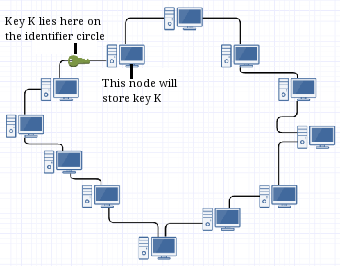
\includegraphics{Selection_152.png}
\caption{\label{family}The identifier circle and a storage of a key k into some node n.}
\label{1}
\end{figure}

Consistent hashing techniques will be used to assign every node in the system an m-bit identifier. The SHA-1 hash on every node’s IP address is calculated, and this value is used as that node's unique identifier. For files, the SHA-1 hash of the file name plus the timestamp that it was created at will also be calculated, which will be used to determine where the file will be stored at initially. The nodes themselves are going to be arranged in an identifier circle (see Fig. \ref{1}). To determine the positioning of a node in the circle, the distance between every other node's identifier (an SHA-1 hash of the IP address) and a particular node's identifier will be calculated to determine which node is the successor or predecessor on the circle.   

Maintaining only a single connection to the successor, while correct, would give a worst case linear runtime for searching a particular key, which is quite inefficient. To alleviate this problem, finger tables \cite{1} will be implemented at each node to keep track of node identifiers and their IP addresses. The ith entry in the table at some node n contains information about the node that succeeds n by at least $2^i - 1$. This means that the first entry is always the immediate successor of that node; hence, it is not required to keep a separate variable to keep track of the successor. The table steps along nodes exponentially so each node only ever needs to keep track of O(log(n)) nodes, where n is the total number of nodes in our network (see Fig. \ref{2}).

Based on the above, where the max degree for each node is upper bounded by log(n), a node, when faced with a query for a key k, will need only lookup the finger table to find a node which is closest to k’s identifier. Then it sends along the request to that node. The next node repeats the procedure recursively, and continues until it reaches a node which holds the key or has a successor which has that key-value pair. This reduces the lookup time to O(logn).

For some SHA-1 hash of a file k, it is stored at a specific node n if it is the very next node (clockwise) starting from the point where key k's identifier lies on the identifier circle (based on the calculated distance between the key k's hash and all the other nodes in the system), or on a node n if in the rare case of a hash collision where the SHA-1 hash of key k is equal to the identifier of n (giving a distance of zero). 

The node numbers will range from 0 to $2^m$ - 1. If a high enough m is chosen, the probability of collisions is lessened.

\begin{figure}[!htb]
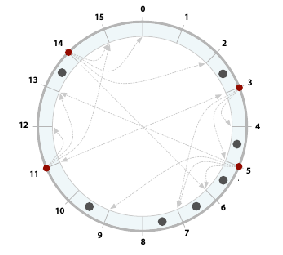
\includegraphics{Selection_155.png}
\caption{\label{family}Overlay network appearance with finger tables \cite{1}. Each node has a finger table which points to some other node. Only the finger tables of the red nodes are shown.}
\label{2}
\end{figure}

\subsection{Node subscription}

\begin{figure}[!htb]
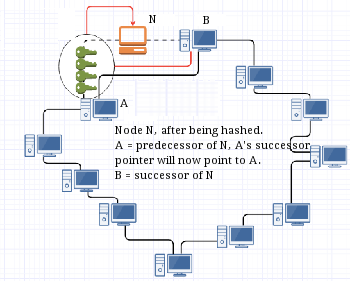
\includegraphics{Selection_153.png}
\caption{\label{family}Node entry case.}
\label{3}
\end{figure}

A joining node will have the SHA-1 hash of its IP calculated to identify a spot on the identifier circle. Once identified, the finger table of the predecessor will be updated accordingly to point to the new node (now its new successor), and recursively through all the finger tables of all the other nodes which had entries for the node that was moved over (now the successor of the new node) in the identifier circle (see Fig. \ref{3}). Certain keys in the new node’s successor will now be transferred over to the new node (specifically the keys that fall between n’s predecessor and n). 

\subsection{Node exit and failures}

\begin{figure}[!htb]
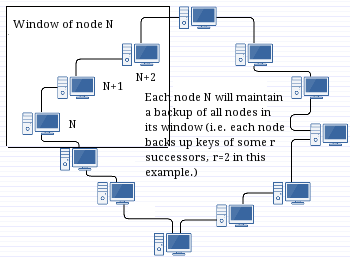
\includegraphics{2016-02-29.png}
\caption{\label{family}Node exit/failure case.}
\label{4}
\end{figure}

If a node fails/leaves all of its keys will be reassigned to it’s successor (see Fig. \ref{4}). The finger tables will also be updated recursively, removing every entry which previously held the exited node.

To deal with unexpected failures/a high churn rate and minimize the probability of data loss, every node in the circle will keep track of a subset arc of our identifier circle. For example, node n will maintain backups for node n+1, n+2 and n+3. So if in the near future, node n+2 fails, node n will be able to recover data (and send it to node n+4 since it’s the next best candidate for storing all of n+3’s keys). This window of backups shall be maintained for every node in our network, allowing for quick recoveries. The replication factor r (see Fig. \ref{4}) is decided beforehand as possibly an argument to the go program, but this will generate a certain number of backups that should ideally scale to O(logn).

To detect failures, heartbeat messages will be sent from predecessor to successor, where for every 2 arbitrary messages to the successor, the predecessor will expect one back - if no reply was detected, then assume the node is lost and update the finger tables accordingly.

\subsection{Media streaming and delivery}

Given that some nodes have stored in them a multimedia file, such as video, when the client wants to stream a video from its peers, it will do a lookup on the finger table to obtain the id of the node that has the file. Once a node is obtained, a lookup on the finger table of that node for another node that has the video file will be done. In doing so, once a certain number of nodes for the file is obtained, a stream to the video is initialized, which will be done in terms of a sequence of frames. 

A queue to store a list of all the frames of the video will be used and we will keep asking the connected nodes for the frames in sequence. In the case where a later frame is obtained sooner than an earlier frame, the frame is stored in a buffer and the playback of the frames will occur only once an ordered sequence has been obtained. 

In the case where nodes that were sending frames die or leave the network, the frame requests are redistributed across other available and connected nodes. In the case where all nodes except for the client are lost, lookups on the finger table will be performed for live nodes that contain the file, and once at least one live node is obtained, send the node the frame request again. This assumes consistency across all the nodes in terms of finger tables.

\subsection{Challenges and related issues}

In constructing this system, therein lies a significant challenge with regards to maintaining consistency due to dynamic structural changes that is caused primarily by high rates of churn. In order to maintain the ring structure, the original Chord paper \cite{2} suggests a protocol where each node periodically checks if its successor is still alive and updates their finger table accordingly (see Fig. \ref{5}).

\begin{figure}[!htb]
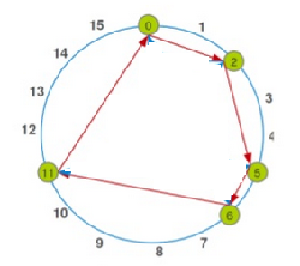
\includegraphics{stabilize1.png}
\caption{\label{family}Handling peer churn. The correct successor is the first node that is found to be alive by traversing in the clockwise direction (red arrows).}
\label{5}
\end{figure}

This detection and notification will be run in the background using go routines and heartbeat messages (to test for abrupt disconnections, as explained in section 2.3).

There are also a number of papers attempting to use a simplified Paxos consensus algorithm adapted into DHT to enhance consistency and reliability \cite{2} \cite{1}. Although this is slightly beyond the scope of this system, experimenting with this approach as a strategy to deal with the dynamism of this P2P system would serve it well.

\section{Project Timeline}

To allow as much time as possible for polishing, debugging, and unforeseeable events, the basic construction of the identifier circle of nodes, which handles joining and leaving cases should be completed by Mar. 18, which corresponds to the project status meeting date. The media streaming section will take on most of the bulk of the project in terms of effort and time, and thus should be accommodated accordingly. To follow good industry practices, this group will probably follow test driven development (TDD) and SCRUM methods throughout the development of the project, so that feature implementation is planned and executed with minimal risk. In this section the GUI will be implemented, and the project will be hosted on a free website, possibly Heroku. It is hoped that any user can then upload multimedia content to some centralized server, of which other users can then stream using this group's implemented system.

\section{SWOT Analysis}

\subsection{Strengths}
A lot of research material is available in regards to the Chord DHT implementation as well as several available lectures and notes on the subject.Additional strengths include disciplined team members as well as flexible and open meeting hours. Team members are also familiar with other programming languages such as C, Java, C++, Python, Ruby, Prolog and Haskell, and so code optimization ideas can be transferred over from that knowledge of other languages.

\subsection{Weaknesses}
The system will be difficult to test for a large number of nodes due to limited availability of resources such as a large number of computers/nodes which would be used to test our system under ideal conditions. A significant weakness is that all team members are completely new to distributed systems and as a result, implementation of features of the system will require a lot of additional research and testing.

\subsection{Opportunities}
The Go programming language was created to specifically build distributed systems. As was seen in the class assignments, standard networking procedures are fairly straightforward to implement using this language. As such the programming language itself provides the group with a lot of opportunities to focus on the implementation of the distributed system itself rather than spend a lot of time on implementing the basic networking required for the system.

\subsection{Threats}
The Go programming language is fairly new which makes well established solutions to specific problems harder to come by than other languages. Furthermore, the members of this group have not had experience with it prior to taking this course, and as such, the best practices and idioms that come with this language will not come as intuitively. 

\section{Conclusion}

A possible solution to the drawback of the centralized client-server model in media streaming can be found through the use of a P2P network. This is achieved by sharing the bandwidth requirements across several disjoint nodes which serve to forward the data stream among themselves, not over one singular connection. Such a system is complicated to build however, and gives rise to its own set of disadvantages. Peer churn in particular, remains a significant challenge and one that is still not adequately addressed with most current P2P implementations.

\phantomsection
\bibliographystyle{unsrt}
\bibliography{sample}

%------------------------------------------------

\end{document}